\chapter{Temperature distribution} % of an L-shaped structure}

\modinfo{Directory}{TemperatureAngle}
\modinfo{Solvers}{\Idx{HeatSolve}} 
\modinfo{Tools}{\Idx{ElmerFront}} 
\modinfo{Dimensions}{2D, Steady-state}

\subsection*{Problem description}

An L-shaped structure (see figure~\ref{fg:struct1}) is heated by an
internal heat source, which magnitude is 1 W/m$^3$. The density of the
structure is 1 kg/m$^3$ and the heat conductivity is 1 W/mK. All the
boundaries $\Gamma_i$ are kept on constant temperature of 0 K. The
problem is to solve the temperature distribution in the structure.

\begin{figure}
\begin{center}
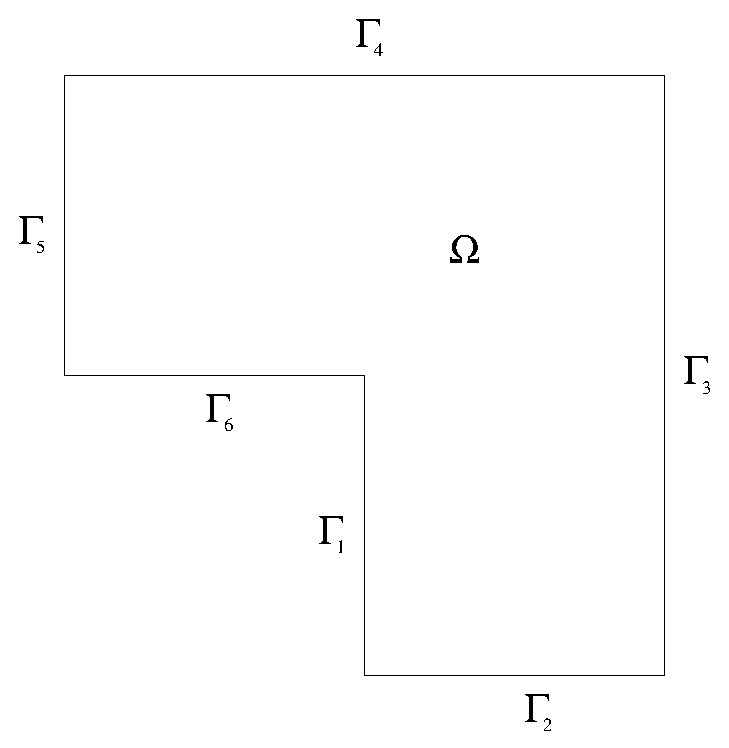
\includegraphics[width=60mm]{Area1}
\caption{L-shaped structure}\label{fg:struct1}
\end{center}
\end{figure}

Mathematically the problem to be solved is
\begin{equation}
\left \{
\begin{array}{cccc}
- \kappa \Delta T &= &f & \mbox{ in } \Omega \\
T&=&0 & \mbox{ on } \Gamma
\end{array}
\right .
\end{equation}
where $\kappa$ is the heat conductivity, $T$  is the temperature 
and $f$ is the heat source. It is assumed that density 
and heat conductivity are constants. 

\subsection*{Solution procedure}

\begin{itemize}
\item Start Elmer in the desired directory with the command 
\ttbegin
ElmerFront
\ttend
\item Open the file that contains the geometry of the structure from 
the File menu. Select also the working directory for the model.
\ttbegin
File -> Open cad-file 
  File = TempDist.egf 
  Model name = TempDist 
  Model directory = temp_tutorial
\ttend
\item Select the equations to be solved from the Problem menu. In this 
case there is only one equation, the heat equation. 
\ttbegin
Problem -> Equations 
  Heat equation 
\ttend
\item Apply the body forces from the Model menu. Give the value for the body 
force (heat source). 
\ttbegin
Model -> Body forces 
  Heat source = 1
\ttend
\item Define the material properties from the Model menu. Give the values for 
the density and the heat conductivity. 
\ttbegin
Model -> Materials 
  Density = 1 
  Heat conductivity = 1
\ttend
\item Define boundary conditions from the Model menu. Give the value of the 
temperature at all boundaries $\Gamma_i (i=1,\ldots,6)$.
\ttbegin
Model -> Boundary conditions 
  Temperature = 0 
\ttend
\item Define mesh for the structure from the Mesh menu. First give name for 
the mesh and then define the element size. Press finally the ``Generate 
Mesh'' button.
\ttbegin
Mesh -> Define mesh 
  Mesh name = Mesh1 
  Model Mesh H [m] = 0.1 
  Generate mesh
\ttend
\item Now the problem may be solved.
\ttbegin
Run -> Solver 
\ttend
\item After the solution is done, view the results by selecting the 
Postprocessor from the Run menu. 
\ttbegin
Run -> Postprocessor 
\ttend
\item To save the created model, select Save model file from the File menu.
\ttbegin
File -> Save model file 
\ttend
\end{itemize}

\subsection*{Results}

As a result the maximum temperature in the structure is given. For a
comparison the same problem was solved six times with different
element sizes. The maximum temperature obtained by using different
meshes is recorded in Table~\ref{tb:struct1}.  From the results one
can see that the result converges. With a denser mesh the result is
more accurate, but solving the problem takes more calculation time.
For reference, the central processor (cpu) time used in each case is
also shown in the table.

\begin{table}
\caption{Results with different element sizes}
\label{tb:struct1}
\begin{center}
\begin{tabular}{llll} \hline
Model Mesh H [m]  & Elements & $\max (T)$ [K] & cpu time [s]\\ \hline
0.2 & 187 &  0.1452  & 0.25 \\
0.15 & 330 & 0.1462  & 0.28 \\ 
0.1 &  735 & 0.1478  & 0.38 \\
0.05 & 2793 & 0.1487  & 0.85 \\ 
0.025 & 11100 & 0.1492 & 2.88 \\ 
0.01  & 69654 & 0.1493 & 19.37 \\ \hline
\end{tabular}
\end{center}
\end{table}

\hfill



